%! TEX root = ../msc.tex
\chapter{Introduction}
\label{ch:basics}
\epigraph{I am fascinated by numbers}{
\citeauthor{baron-cohenAutismSpectrumQuotientAQ2001}}
%\cite{baron-cohenAutismSpectrumQuotientAQ2001}}

Was hier useful werden kann:

Nielsen: \cite{nielsenQuantumComputationQuantum2010}

Stabilizer Formalism, Gottesman PhD thesis: \cite{gottesmanStabilizerCodesQuantum1997}

Algorithm for simulating stabilizer circuits:
\cite{aaronsonImprovedSimulationStabilizer2004}

stabilizer lecture notes: \cite{arabLectureNotesQuantum2024}

Entanglement with Stabilizers: \cite{fattalEntanglementStabilizerFormalism2004}

Aaronson's quantum information theory I and II lecture notes:
\cite{aaronsonIntroductionQuantumInformation,aaronsonIntroductionQuantumInformationa}.
This one's a huge find!

This chapter serves to familiarize the reader with the core concepts relevant
to this thesis. We will first introduce the stabilizer formalism, as it will
later enable us to perform efficient numerical experiments on a classical
computer. We then provide a general introduction to the field of entanglement
transitions and go over some important examples. 
\section{The Stabilizer Formalism}\label{sec:stab-basics}
In this section we review the most important concepts of the stabilizer
formalism. 

Section adapted from \cite{nielsenQuantumComputationQuantum2010} and
\cite{gottesmanStabilizerCodesQuantum1997}
\subsection{Basic notions of group theory}
blabla

\begin{defn}\label{defn:fixpointgroup}
  Let $G$ be a group acting on a set $M$. Let $a\in M$. We then call the
  subgroup
  \[ H = \left\{ h \in G \mid ha = a \right\} \leq G \]
  \emph{symmetry group} or \emph{fixpoint group} of $a$.
\end{defn}


Consider the 2-qubit Bell state
\begin{align}
  \ket{\psi} = \frac{\ket{00} + \ket{11}}{\sqrt{2}} 
.\end{align}

Note that the unitary operations $X_1 X_2$ and $Z_1 Z_2$ both have $\ket{\psi}$
as eigenstate with eigenvalue $+1$.


\begin{defn}
  Let $S\leq G_n$. We define $V_S$ as the set of $n$ qubit states stabilized by
  $S$.
\end{defn}

Currently verbatim from \cite{nielsenQuantumComputationQuantum2010}! Beware!
Actual source is \emph{inside}
\cite{gottesmanHeisenbergRepresentationQuantum1998}, basically stating "trust
me bro" (one of the most important theorems of quantum computation is cited as
private communication in its original source\ldots)
\begin{thm}[Gottesman-Knill theorem]\label{thm:gottesman-knill}
  Suppose a quantum computation is performed which involves only the following
  elements: state preparations in the computational basis, Hadamard gates,
  phase gates, controlled-\verb|NOT| gates, Pauli gates, and measurements of
  observables in the Pauli group (which includes measurement in the
  computational basis as a special case), together with the possibility of
  classical control conditioned on the outcome of such measurements. Such
  computation may be efficiently simulated on a classical computer.
\end{thm}
We will forego a detailed discussion of \cref{thm:gottesman-knill} until
\cref{sec:tableau}. 

\section{Entanglement Transitions}\label{sec:ent-trans}

Random assortment of MIPT Paper (incomplete):

\begin{itemize}
  \item Fisher paper, das ich mir als allererstes mal durchgelesen hab
    (\citetitle{liMeasurementdrivenEntanglementTransition2019}):
    \cite{liMeasurementdrivenEntanglementTransition2019}
  \item MIPT general, war in \cref{ch:lxe}, aber leider keine ahnung mehr
    warum\ldots (\citetitle{baoTheoryPhaseTransition2020}) \cite{baoTheoryPhaseTransition2020}
  \item \citetitle{baoSymmetryEnrichedPhases2021}
    \cite{baoSymmetryEnrichedPhases2021}
  \item Why not: Measurement induced synchronization von Finn
    (\citetitle{schmolkeMeasurementinducedQuantumSynchronization2023}):
    \cite{schmolkeMeasurementinducedQuantumSynchronization2023}
  \item 2017 WR for quantum state tomography (10 qubits):
    (\citetitle{song10QubitEntanglementParallel2017})
    \cite{song10QubitEntanglementParallel2017}
  \item LXE: Definition: \cite{liCrossEntropyBenchmark2023}; PTIM:
    \cite{tikhanovskayaUniversalityCrossEntropy2023}
  \item Garratt/Altman Paper:
    (\citetitle{garrattProbingPostmeasurementEntanglement2023}) \cite{garrattProbingPostmeasurementEntanglement2023}
  \item self-cite for clout:
    (\citetitle{schmolkeBoostingInformationTransfer2024})
    \cite{schmolkeBoostingInformationTransfer2024}
\end{itemize}
\begin{figure}[H]
  \centering
  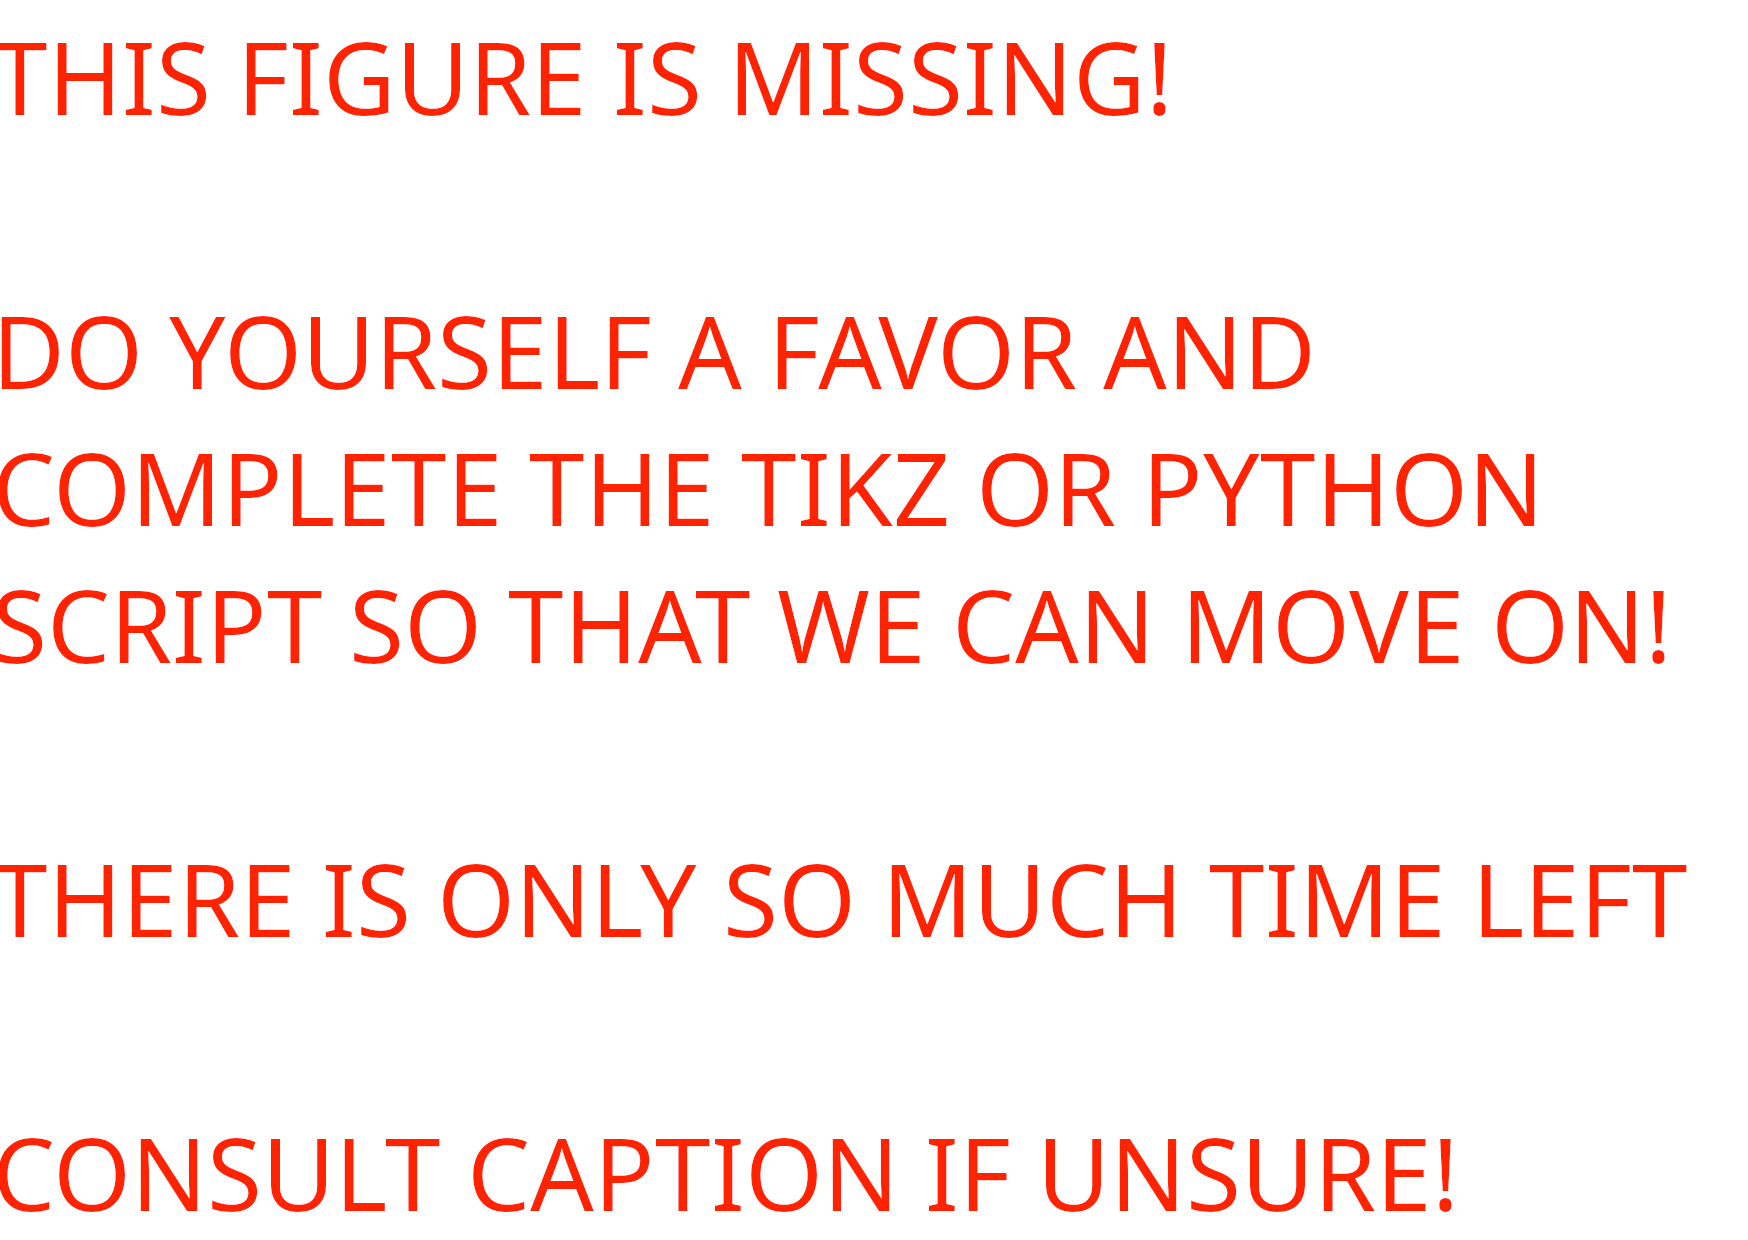
\includegraphics{Untitled.png}
  \caption{Hybrid Circuit Tikz picture??}
  \label{fig:hybrid-circuit}
\end{figure}

\subsection{Phenomenology}

\section{The Projective Transverse-Field Ising Model}
\begin{itemize}
  \item PTIM paper: \citetitle{langEntanglementTransitionProjective2020}
    \cite{langEntanglementTransitionProjective2020}
  \item Felix decoder paper: \citetitle{roserDecodingProjectiveTransverse2023}
    \cite{roserDecodingProjectiveTransverse2023}
  \item Colored Cluster Model!
  \item There should be a Skinner paper, but I don't have it in my zotero
    library (yet)
\end{itemize}

\begin{figure}[H]
  \centering
  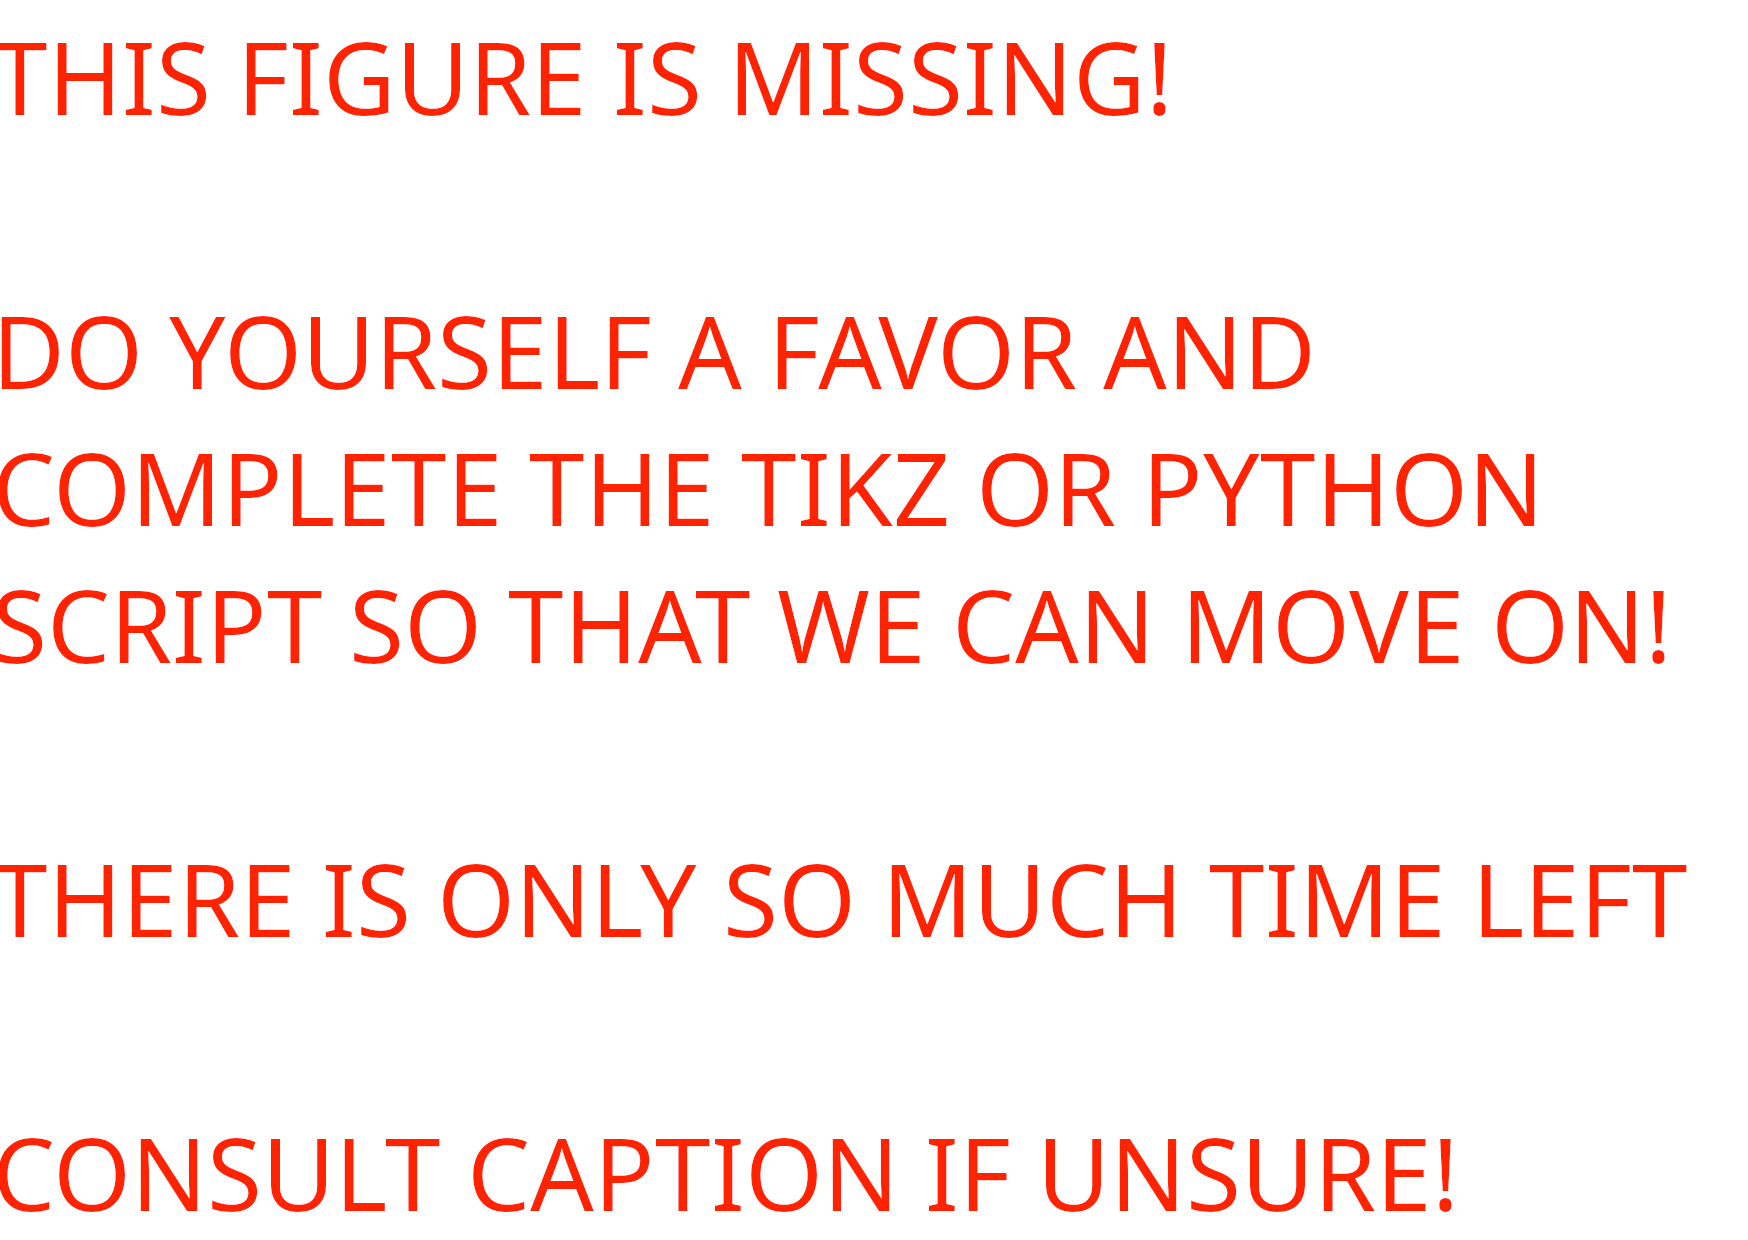
\includegraphics{Untitled.png}
  \caption{Tikz sketch of PTIM setup with $\approx 10$ qubits}
  \label{fig:ptim-circuit}
\end{figure}

\begin{figure}[H]
  \centering
  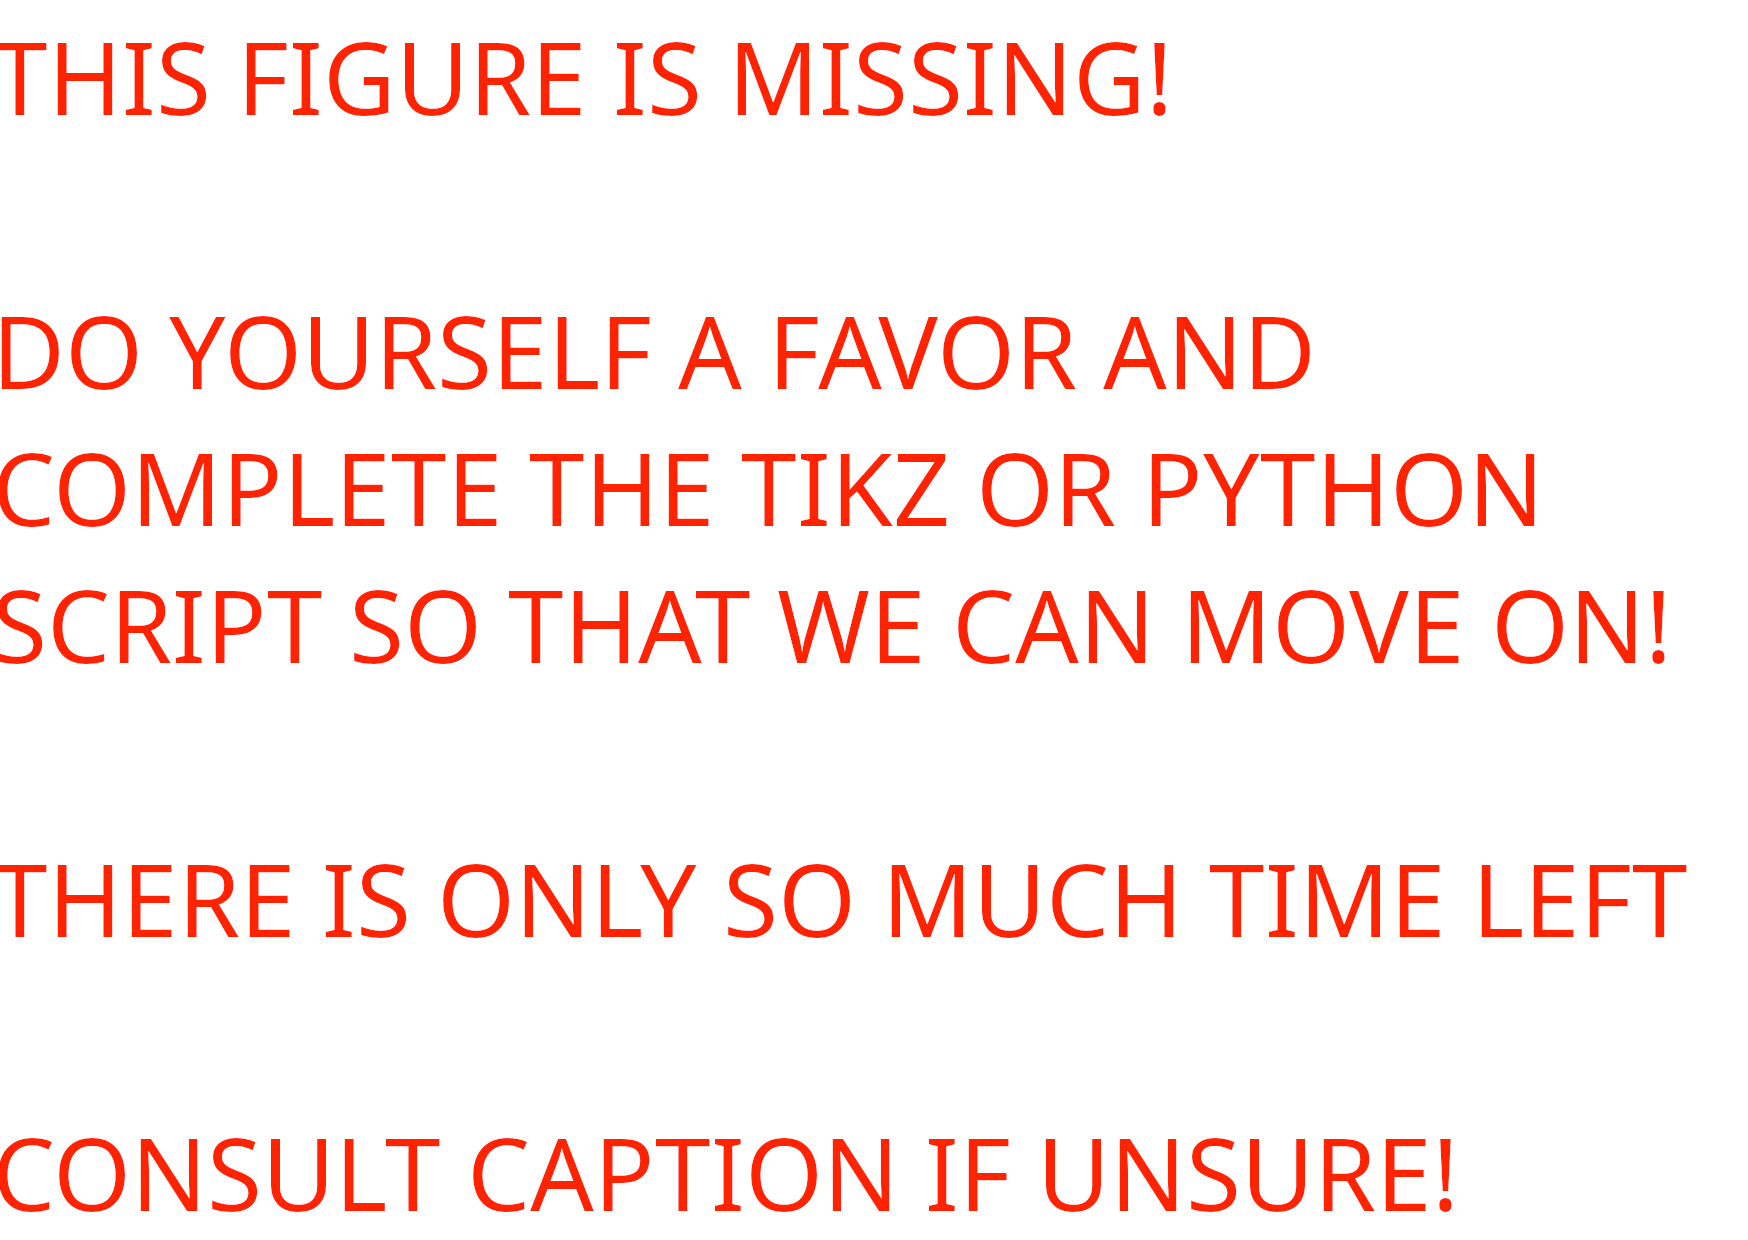
\includegraphics{Untitled.png}
  \caption{plot of entanglement entropy (and mutual information??) as a
  function of $p$. multiple system sizes, possibly rather large ($\approx 512$
qubits?, maybe $N=\{128,256,512\}$ just for the fun of it). Would need to
include mutual information in the source code.}
  \label{fig:phase-transition}
\end{figure}

\section{Sampling Problem}\label{sec:sampling}
The metaphysics of this endeavour can
be condensed in the following way; we (a) know from experiments how quantum
systems behave under certain conditions, and (b) predict through theoretical
calculations what these systems might do in another experimental setting. In
the latter case however, there is an uncanny regime of utility, where we either
(a) cannot precisely pass predictions or (b) cannot perform the experiment on
the grounds of hardware limitations\footnote{The Higgs particle was predicted
40 years before it was discovered \textcolor{red}{citation}} or (c) try to
predict the behavior of quantities not directly measurable. In the case of
quantum computation, and especially in the field of entanglement transitions,
we face these bottlenecks in increasing severity. To make do with them, we
employ classical computer simulations. That is, we perform numerical
experiments. While traditional experiments still serve as the sole proprietor of claim to
ontology, numerical experiments can play a supporting role, 

In the year of our
lord 2024, we phyisicists are thankfully able to perform experiments at home
with cleverly assembled silicon.  That is, nowadays we make do with these
bottlenecks by performing numerical experiments. This is not to discredit the
utility of experiments as such, on the contrary! 

\subsection{Fisher: Linear Cross Entropy}
\cite{liCrossEntropyBenchmark2023}

\subsection{Altman: Upper Bound}
\cite{garrattProbingPostmeasurementEntanglement2024}
